\newpage
\section{Irradiation studies of the powering units}
Radiation-induced effects in electronics play an important role in accelerator facilities, where different particle species may elevate radiation levels even in relatively remote areas. Depending on many factors, i.a. location of the setup, intensity or energy of the incident particles, damage caused to a semiconductor device may vary greatly. A particle could cause no observable effect, transient disruption of circuit operation, a change of logic state, or even permanent damage to the device or integrated circuit (IC)~\cite{dodd}. The detector will be powered by about 140 low voltage modules, providing 2100 power channels. In order to estimate the Single Event Effects (SEE) in the powering electronics in the envisaged radiation environment, two irradiation campaigns took place in GSI, Darmstadt.  The first one was conducted at the mini-CBM experiment and the second was realized next to the electrostatic septum of the SIS18 synchrotron. These irradiation campaigns aimed at detecting radiation-induced soft errors in the power units' electronics and estimating its rate.


\subsection{Single Event Effects in the electronics}
A variety of different elements and chemical compounds can be used in electronics, including silicon, silicon dioxide ($\mathrm{SiO}_{2}$), or boron. The high ambient flux of particles in a particle accelerator environment usually consists of charged particles (mostly protons, and electrons), high-energy photons (gamma and X-rays), and a broad spectrum of neutrons. Different interaction mechanisms may cause both stochastic and deterministic effects in electronics. These effects are directly related to the integrated dose and linear energy transfer (\gls{LET}) of the incident particles ~\cite{electronic_system_on_module}. Radiation-induced soft errors have become a huge concern in advanced computer chips because uncorrected, they produce a failure rate that is higher than all the other mechanisms compromising reliability combined~\cite{1545891}. Neutrons do not cause direct ionization in silicon or oxygen. These neutral particles interact elastically as well as inelastically, resulting either in the creation of other nuclei and the emission of a light particle or in changes in the kinetic energies of the participants. A few neutron threshold energies for reactions with oxygen and silicon are summarized in Table~\ref{cross-seciton}. The cross-section for neutron reactions generally decreases with the energy. Moreover, neutrons can indirectly cause SEE by secondary radiation, for example, a reaction with boron which results in the emission of an $\alpha$ particle $^{10}\mathrm{B}(n,\alpha)^{7}\mathrm{Li}$~\cite{1545891,neutrons_energy,neutrons_energy_2}. 

\begin{table}[!h]
\centering
\caption{Threshold energies of neutron reactions with silicon and oxygen nuclei~\cite{ENDF}.}
\begin{tabular}{lc}
\hline
Reaction         & Neutron Threshold Energy (MeV) \\ \hline
Si elastic       & 0                              \\
Si(n,$\alpha$)   & 2.75                           \\
Si(n,p)          & 4                              \\
Si(n,d)          & 10.5                           \\
Si(n,$n-\alpha$) & 10.35                          \\ \hline
O elastic        & 0                              \\
O(n,$\alpha$)    & 2.35                           \\
O(n,$n-\alpha$)  & 7.61                           \\
O(n,p)           & 10.24                          \\
O(n,d)           & 10.53                         
\end{tabular}

\label{cross-seciton}
\end{table}

\newpage
\subsection{Motivation}

The powering of the Front End Boards (\gls{FEB}s), together with the data processing electronics, sum up to about 2100 low voltage channels, operated in about 140 low voltage modules, 16 channels each. All of them will be placed in a protected area within the cave with an elevated radiation level. The estimated dose values were calculated by A. Senger using FLUKA code (see Figure~\ref{fig:mCBM})~\cite{FLUKA}. 

\begin{figure}[!h]
    \centering
   % 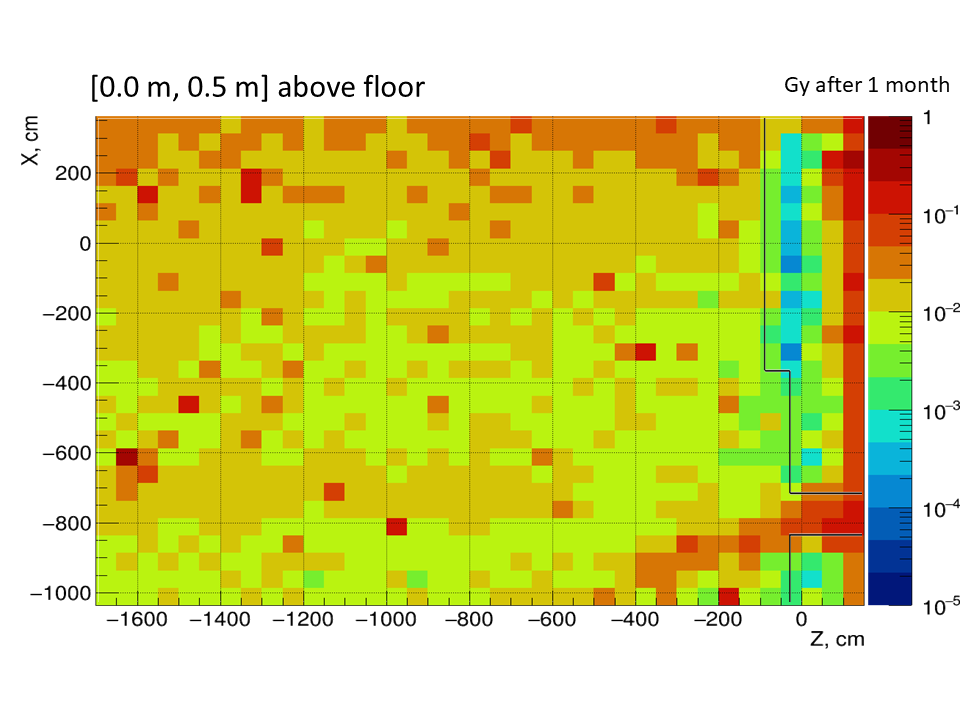
\includegraphics[width=0.95\columnwidth]{images/dose3.png}
    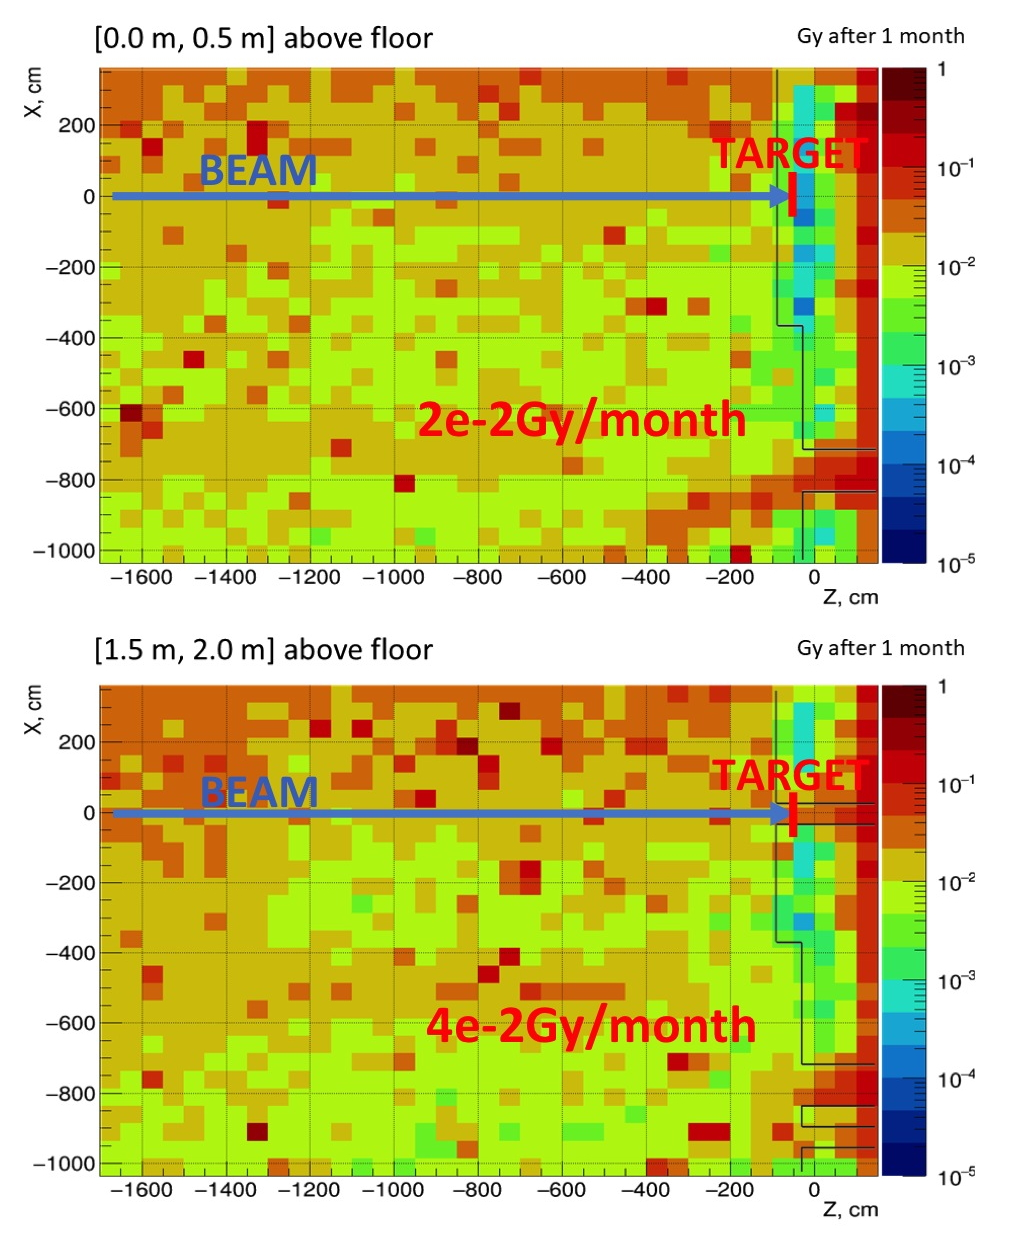
\includegraphics[width=0.55\columnwidth]{Chapter4/images/Dose00.jpg}
    \caption{Expected dose distribution in the air in the \gls{CBM}
cave under the platform in (11 AGeV Au $10^{9} \mathrm{\ ions/s}$ on 1\% Au
interaction target) 0 to 0.5 m and 1.5 m to 2 m above the ground} 
    \label{fig:mCBM}
\end{figure}
%\newpage
For the gold beam with the highest available intensities ($10^{9}\mathrm{\ ions/s}$) and energies (11 AGeV), we expect a total dose level of 20 \footnote{Gray is a SI unit of ionizing radiation dose, defined as the absorption of one joule of radiation energy per kilogram of matter \cite{gray}}{mGy} after 1 month of operation in the area between 0 and 0.5 m above the ground (at the planned location of the power crates x = -600 cm, z = -600 cm) and 40 mGy between 1.5 m and 2 m above the ground (x = -600 cm, z = -600 cm). A failure in the low voltage powering of the FEE may lead to a rapid decrease of temperature, as the primary coolant temperature may reach down to $-40^{\circ}\mathrm{C}$, consequently making the FEE susceptible to thermal stress. The effects of radiation must be therefore studied to ensure the safe operation of the STS. Estimation of the soft error rate (\gls{SER}) may also indicate whether there is a need for further shielding of the power electronics in order to minimize the overall dose.

\newpage
\subsection{Methodology}
The subject of the irradiation campaign was a MPOD mini crate with one low voltage (WIENER) and one high voltage (ISEG) module. The crate's CC24 controller (ISEG) offers an embedded \gls{EPICS} Input Output controller, which was used to detect radiation-induced channel or module failures. All registered events were stored in a dedicated database.  In order to correlate the soft failure rate with the absorbed dose, two types of thermoluminescent dosimeters were used. A larger polyethylene sphere (d = 30 cm) was used to measure the neutron ambient dose, whilst the cylinder (d = 5 cm, h = 6 cm) measured other particles~\cite{bonner}. We assume that the conditions (neutron spectra - mostly thermal neutrons, neutron moderators, etc.) at the \gls{CBM} experiment will be similar to conditions at SIS18, and at the mCBM experiment. Therefore, the quality factor, which takes into account both \gls{LET} and relative biological effectiveness (\gls{RBE}), to convert the measured given in Sv to absorbed energy in Gy is 5 for both irradiation campaigns. The dose measured with the cylinder is assumed to have a quality factor of 1.

\subsection{Poisson distribution}
We assume that failure events (radiation-induced errors) are statistically independent and are driven by purely stochastic factors. In addition to that, we take into account only the total dose measured by the dosimeters, thus rapid dose changes and their effect are not investigated in this contribution. In such a case, the probability of observing $n_{m}$ events with the mean value $\mu$ is described by the Poisson distribution:\newline
\begin{equation}
    p(n|\mu) = \frac{\mu^{n}}{n!}e^{-\mu}
\end{equation}
The total number of events is considered to be the average $\mu$, as this is the most reasonable assumption.
Assuming 68\% confidence levels for values $n_{m} > 2$ we can apply the following equations to estimate the distribution's bands (see Figure~\ref{fig:poisson})~\cite{schmidt}.
If in an experiment $\mu$ events are measured, we conclude that the standard deviation is described by $\mu - \sqrt{\mu}$ and $\mu + 1 + \mu$ around the average value $\mu$.
\begin{figure}[!h]
    \centering
    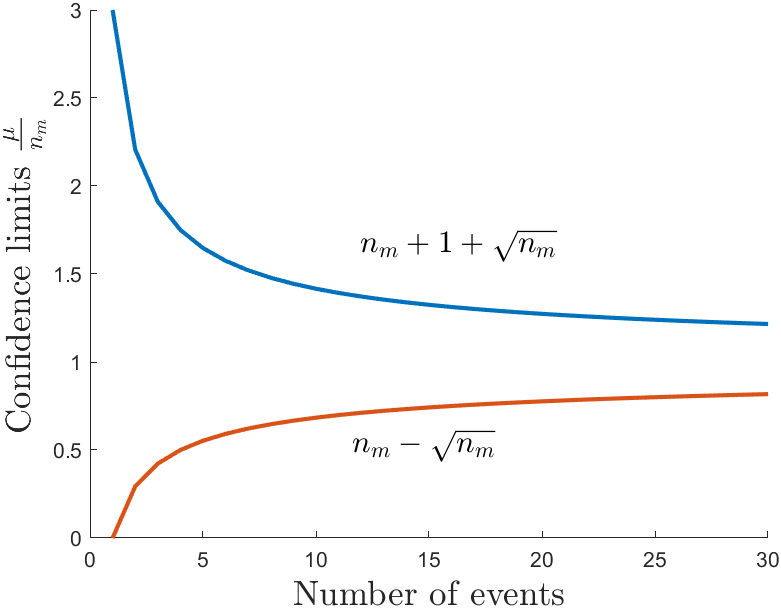
\includegraphics[width=0.55\columnwidth]{Chapter4/images/poisson.png}
    \caption{Estimated bands of the Poisson distribution~\cite{schmidt}}
    \label{fig:poisson}
\end{figure}
%\newpage
For $n_{m} \leq 2$ previously mentioned, estimations do not provide accurate results, therefore upper and lower bands need to be calculated explicitly. According to~\cite{schmidt}:



\begin{table}[!h]
\centering
\begin{tabular}{ccc}
\hline
Number of counts & \multicolumn{2}{c}{Poisonn's distrubution} \\ \cline{2-3} 
$n_{m}$          & $\mu_{l}$            & $\mu_{u}$           \\ \hline
0                & 0                    & 1.84                \\
1                & 0.173                & 3.30                \\
2                & 0.708                & 4.64                \\ \hline
\end{tabular}

\end{table}
\newpage
\subsection{Irradiation at the mCBM experiment}
In order to investigate electronics' operation under the realistic conditions, that low voltage modules will face during the CBM experiment, an irradiation campaign took place at the mCBM experiment (see figure~\ref{fig:CBM1}). Different intensities and reaction systems (Au+Au, Au+Ni, etc.) were exercised during the experiment.
\begin{figure}[!h]
    \centering
    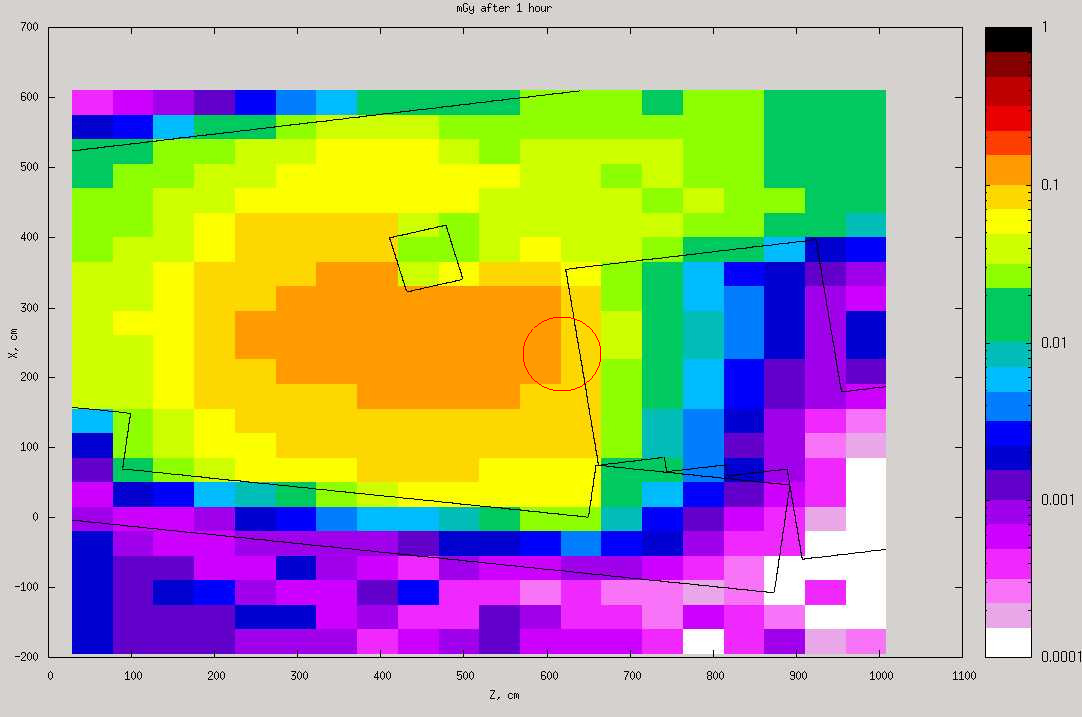
\includegraphics[width=0.65\columnwidth]{Chapter4/images/dose1.jpg}
    \caption{Expected dose rate distribution (mGy/hour) in the mCBM cave with 2 AGeV O ions beam of $10^{7}\mathrm{\ ions/s}$ on 4 mm Ni target. In the encircled area the dose reached about 0.1~mG/hour}
     \label{fig:CBM1}
\end{figure}
\begin{figure}[!h]
    \centering
    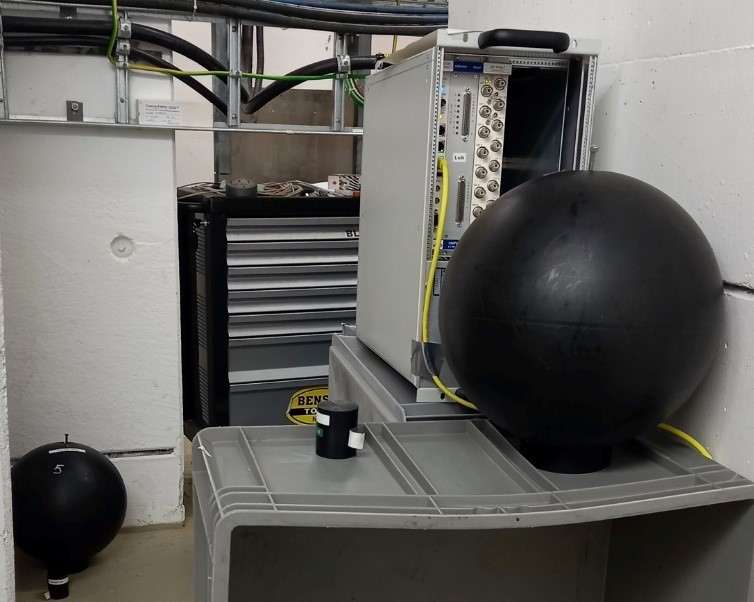
\includegraphics[width=0.5\columnwidth]{Chapter4/images/crate.jpg}
    \caption{Crate irradiation setup at the mCBM experiment. The photo depicts two TLD dosimeters in the background, and two TLD dosimeters and the crate in the foreground}
    \label{fig:crate}
\end{figure}
\newpage
To measure the dose that the crate was exposed to, four thermoluminescent dosimeters (\gls{TLD}) with moderators were used (Figure~\ref{fig:crate}). Two TLDs placed far away from the crate served as a reference. During the irradiation at the mCBM experiment, the dosimeters were read out twice, in order to evaluate the total dose received by the crate. The first value was $19.72\mathrm{\ mGy}$ and  the second one was $72.31\mathrm{\ mGy}$. 

A \gls{SEE} in the low voltage module occurred in each part of the irradiation. In both cases, it was possible to recover the functionalities by enabling the channels again. In total, $n=2$ after ($92\pm{4.6}\mathrm{\ mGy}$), considering standard 5\% uncertainty for the TLD. After applying lower and upper limits we find:
%\newpage
In total, $n=2$ after ($92\pm{4.6}\mathrm{\ mGy}$).
After applying lower and upper limits we get:
\begin{equation}
    D_{lower}=\frac{92}{0.708} = 129.9\mathrm{\ mGy}
\end{equation}
\begin{equation}
    D_{upper}=\frac{92}{4.64} = 19.8\mathrm{\ mGy}
\end{equation}
The uncertainty for $n_{m}=2$ is extremely high and equals to $\mathrm{46}_{-26}^{+84}$ mGy, therefore no clear conclusion on the behavior of the crate could be made. To further increase the statistics, a second irradiation campaign took place at the electrostatic septum of the SIS18 synchrotron. 
%\vspace{10cm}
\subsection{Irradiation at the SIS18 septum}
\subsubsection{Setup}
The setup at the SIS18's septum consisted of two \gls{TLD} dosimeters (for neutrons and other particles separately). Furthermore, the total doses from TLDs were supplemented with readouts from two active dosimeters placed behind the wall (see Figure~\ref{fig:spec_des}). 
\begin{figure}[!ht]
    \centering
    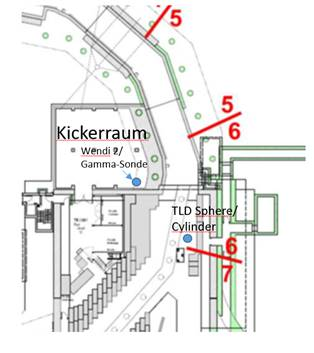
\includegraphics[width=0.45\columnwidth]{Chapter4/images/septum.jpg}
    \caption{Location of the dosimeters and crate at the SIS18. The so-called Kickerraum contained WENDI-2 and Gamma probe, whereas two TLD dosimeters were placed next to the power crate - depicted with a blue dot between segments 6 and 7.}
    \label{fig:spec_des}
\end{figure}

Wendi-2 is a precise wide-energy neutron dosimeter~\cite{wendi} that was used to determine the neutron dose rate in the so-called Kickerraum. Due to the shielding of the wall, the gamma probe measured mostly background radiation. The MPOD mini crate was placed next to the TLD dosimeters. In order to calculate the active neutron dose next to the crate, a ratio of total doses from both measurement places was used. 
\newpage
\subsubsection{Results}
During the irradiation period, readings from the dosimeters reached $106.1\mathrm{\ mSv}$ and $27.7\mathrm{\ mSv}$ for neutrons and other particles respectively.
%(Figure~\ref{fig:spectrum} depicts neutrons spectrum at the irradiation place).
%\begin{figure}[!ht]
%    \centering
%    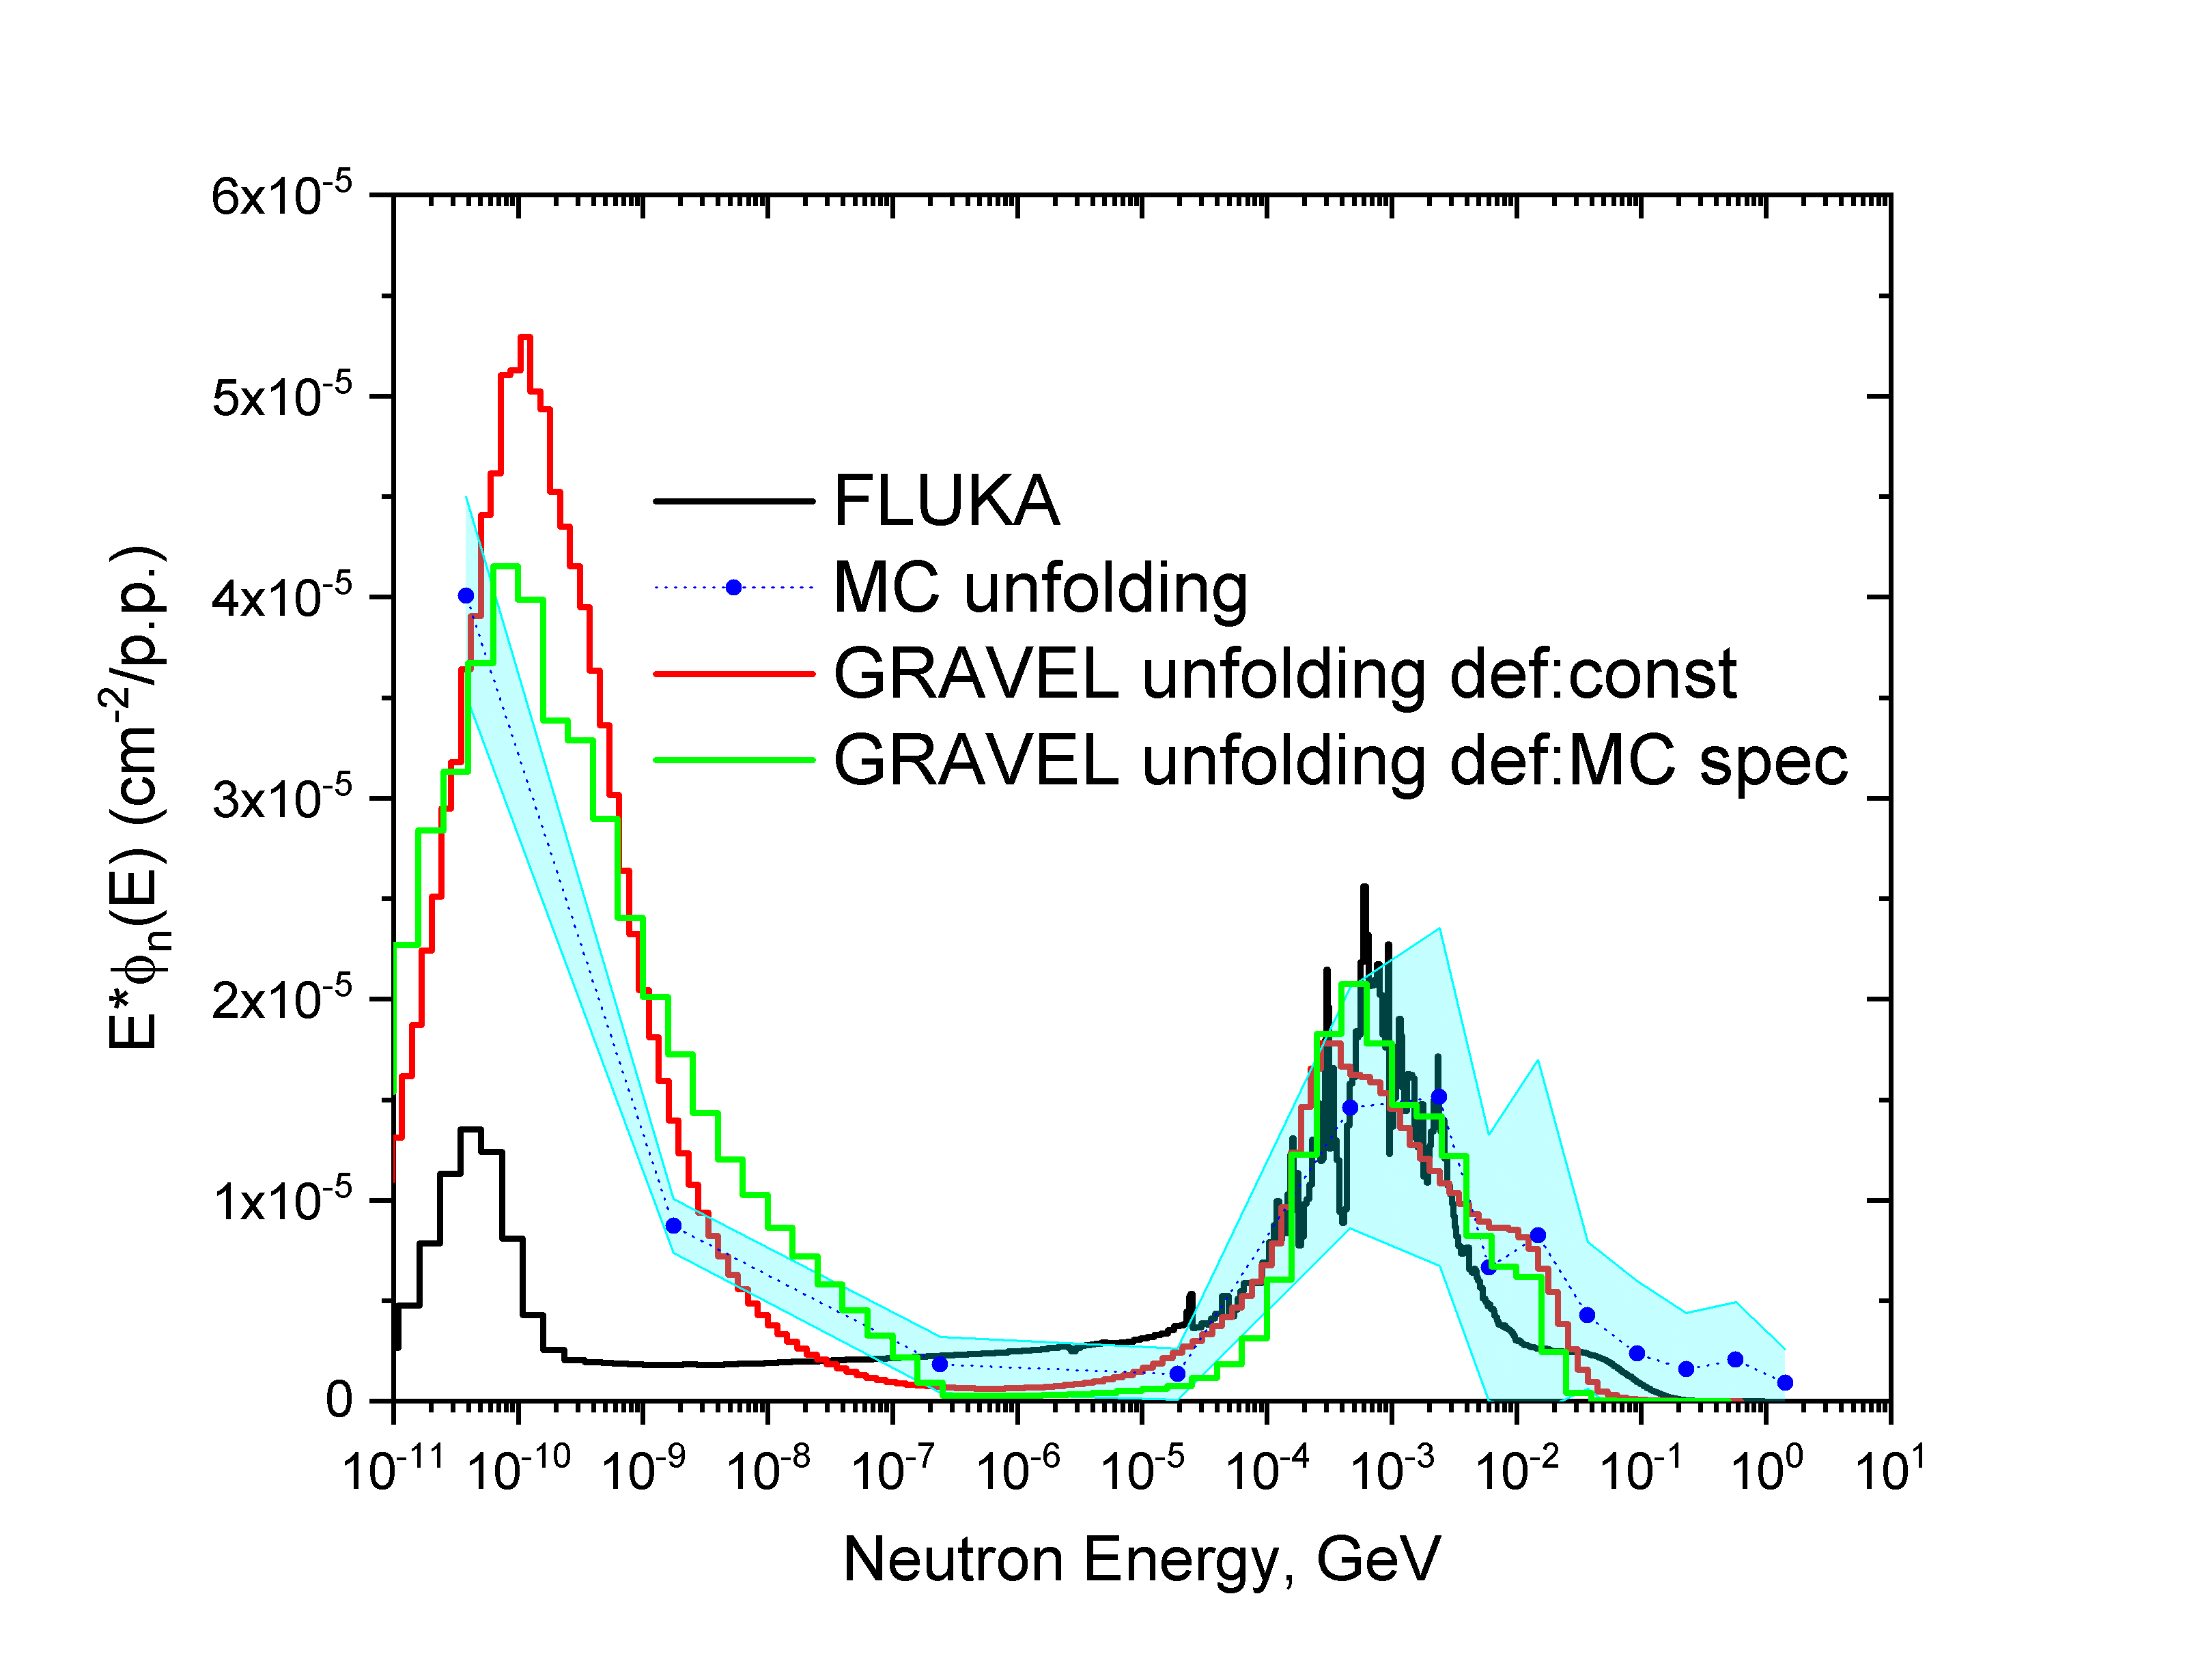
\includegraphics[width=0.9\columnwidth]{Chapter4/images/fig5.png}
%    \caption{Neutron spectrum at the measurement location (SIS18 septum). It is based on the measurement of argon ions at 550 MeV/u. The first peak is related to the thermal neutrons and %the second one to the fast neutrons}
%    \label{fig:spectrum}
%\end{figure}
Using assumed quality factors, we convert the ambient dose to the absorbed dose values. Hence, we get in total $49\pm{2}\mathrm{\ mGy}$, taking into account 5\% standard uncertainty of the TLD dosimeters. During the irradiation 11, radiation-induced soft failures were identified in the low voltage module. Therefore, we can estimate an average dose after which a low voltage failure might take place.
\begin{figure}[!h]
    \centering
    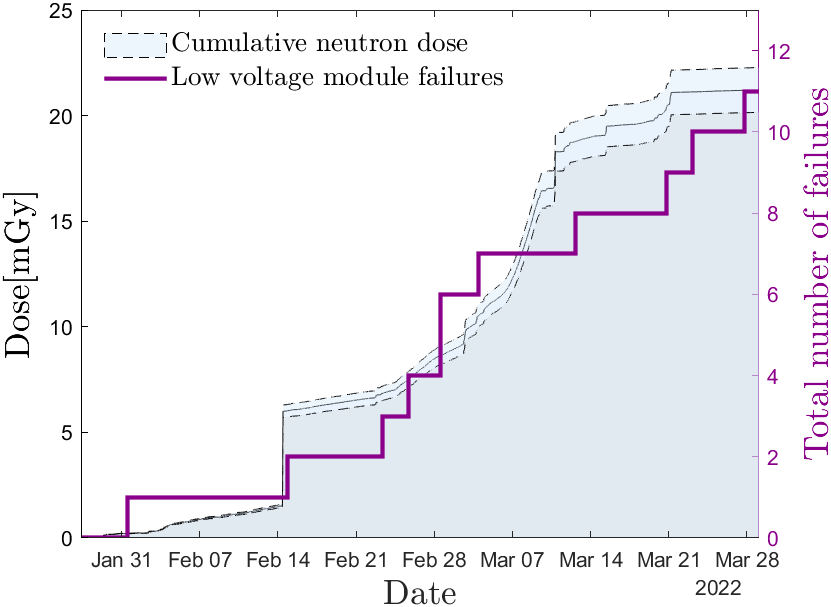
\includegraphics[width=0.6\columnwidth]{Chapter4/images/LV_failure_and_neutronsrate.png}
    \caption{Cumulative neutron dose and SEE in the low voltage module}
    \label{fig:lv_neutrons}
\end{figure}
\begin{figure}[!h]
    \centering
    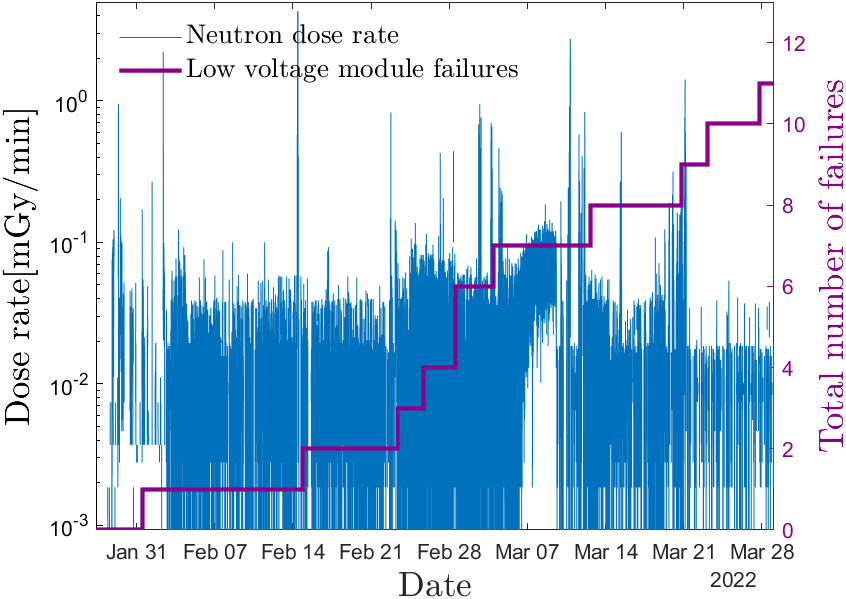
\includegraphics[width=0.6\columnwidth]{Chapter4/images/neutrons_dose_rate.png}
    \caption{Neutron dose rate and failures of the low voltage module}
    \label{fig:lv_neutrons_rate}
\end{figure}
Figure~\ref{fig:lv_neutrons} shows how the number of failures cumulative with the total neutron dose, where the longer periods without failure indicate a break in SIS18 operation. Similarly, Figure~\ref{fig:lv_neutrons_rate} depicts the dose rate and related \gls{SEE}.
For the 11 low voltage module failures, we get the following confidence bands from the Poisson distribution:
   \begin{equation}
  \mathrm{\mu}_{\mathrm{LV}}^{\mathrm{SEE}}=\mathrm{11}_{-3}^{+4}
\end{equation}
Considering the sum of two doses, we get:
\begin{equation}
    \mathrm{D}_{\mathrm{LV}}^{\mathrm{SEE}}=\mathrm{4.45}_{-1.25}^{+1.93}\mathrm{\ mGy}
\end{equation}
Therefore, we can expect a low voltage module failure after $\mathrm{4.45}_{-1.25}^{+1.93}\mathrm{\ mGy}.$ After the occurrence of a soft error in the low voltage module, it was always possible to turn the channels on again.
\newpage
On the other hand, high voltage modules will be placed in an area with lower radiation levels, thus their error sensitivity does not pose a risk to detector operation. In the case of the high voltage module, the \gls{SEE} don't result in a module switch off, but in disabling channels. In two cases all channels were switched off, which is counted as if 15 channels were turned off at the same time. Figure \ref{fig:hv_neutrons} and \ref{fig:hv_neutrons_rate} show the channels' failure rate with the increasing cumulative dose. 
\begin{figure}[!h]
    \centering
    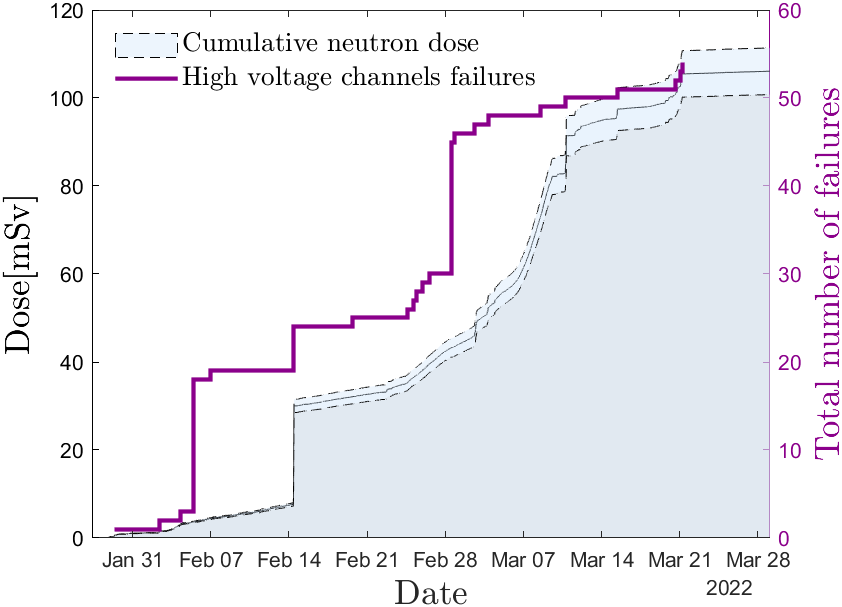
\includegraphics[width=0.6\columnwidth]{Chapter4/images/HV_failure_and_neutronrate.png}
    \caption{Cumulative neutron dose and failures of the high voltage module's channels}
    \label{fig:hv_neutrons}
\end{figure}
\begin{figure}[!h]
    \centering
    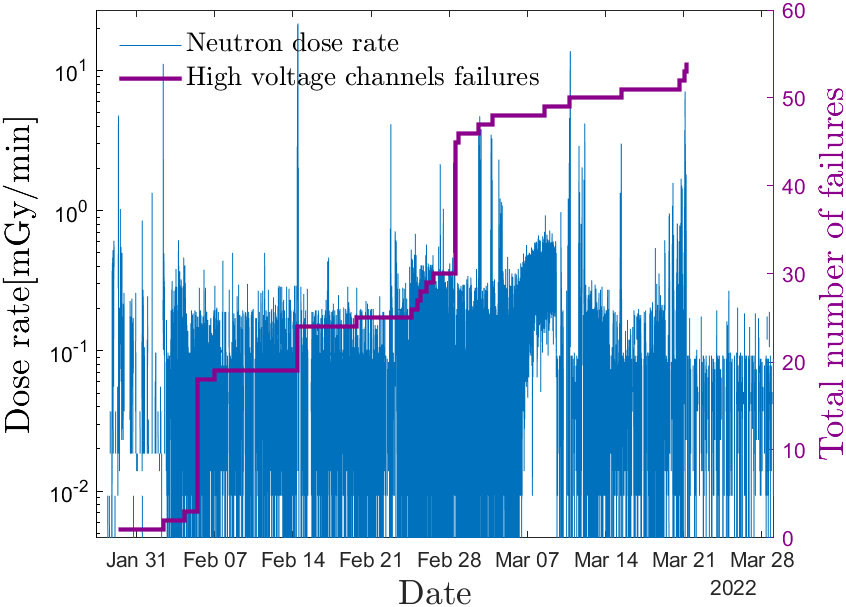
\includegraphics[width=0.6\columnwidth]{Chapter4/images/Hv_neutrons_dose_rate.png}
    \caption{Neutron dose rate and failures of the high voltage module's channels}
    \label{fig:hv_neutrons_rate}
\end{figure}
For the high voltage module, the total number of channels that switched off due to the irradiation is 54. Following a similar procedure as for the previous calculation:
  \begin{equation}
 \mathrm{\mu}_{\mathrm{HV}}^{\mathrm{SEE}}=\mathrm{54}_{-7}^{+8}
\end{equation}
Considering the failure number, it translates to:
\begin{equation}
    \mathrm{D}_{\mathrm{HV}}^{\mathrm{SEE}}=\mathrm{0.91}_{-0.12}^{+0.13}\mathrm{\ mGy}
\end{equation}
If the high voltage module was situated in the same place as the low voltage, we could expect a channel to switch off after $\mathrm{0.91}_{-0.12}^{+0.13}\mathrm{\ mGy}$.
\subsection{Conclusions}
\label{irradiation_results}
The \gls{FEE} of the \gls{STS} will be powered by about 140 low voltage modules. Given that in the worst case some of those modules will be exposed to about 40 mGy/month, the measurement indicates that we can expect about 9 SEE per month per module. In practice, it means that every FEB will need to withstand 9 power cycles at low temperatures per month. Assuming operation of 2 months per year and a total projected operating time of 10 years, electronics must withstand at least 180 power cycles. 
\subsection{Potential risk to operation}
If every low voltage module turns off 9 times per month during the operation, the potential consequences need to be carefully assessed. By planning the powering scheme for the STS, we can prepare the system for the foreseen power interruptions. In the worst-case scenario, considering that we will use 140 low voltage modules, we can expect about 1260 soft errors a month, which means 1.75 errors per hour.  If there were 16 ROBs connected to one low voltage module, we could experience a temporary shutdown of up to 140 FEBs or 70 modules per hour.  The duration of the shutdown is also critical for the operation. A soft error in the low voltage module can most likely be recovered within seconds, preventing extensive thermal stress in the FEE. On the other hand, for the testing scenarios, we need to consider that the electronics experience full thermal stress, in case fast power recovery is not possible. Additionally, power cycles of the FEE in low temperatures may result in thermally induced mechanical stresses on the components of the PCBs. Hence, the effects of thermal cycling of the FEE should be carefully studied, in order to evaluate the limits in the performance of the electronics  (see section~\ref{thermal_cycling}). Nevertheless, there are also a few methods to decrease the potential risk, both from the radiation-induced damage and potential problems due to thermal shock:
\begin{itemize}
    \item additional radiation shielding material around the power supplies,
    \item powering scheme - for example connecting ROBs and corresponding FEBs to the same low voltage module,
    \item proper software/hardware mechanisms to switch on the channels in a timely manner.
\end{itemize}

